\documentclass[10pt,aspectratio=169]{beamer}

\usetheme[progressbar=foot]{metropolis}
\AtBeginSection{}

\usepackage{appendixnumberbeamer}
\usepackage{booktabs}
\usepackage[scale=2]{ccicons}
\usepackage{tabularx}
\usepackage{tikz}
\usetikzlibrary{arrows.meta,positioning,shapes.geometric,fit,calc}
\usepackage{xspace}
\newcommand{\themename}{\textbf{\textsc{metropolis}}\xspace}
\usepackage{comment}
\usepackage{caption}
\usepackage[
  backend=biber,
  style=authoryear
]{biblatex}

\setbeamertemplate{bibliography item}{}
\addbibresource{bibliography.bib}

\usepackage{graphicx}
\usepackage{siunitx}



%................................................................................
% COLORS

\definecolor{ukudlaBlue}{RGB}{41, 60, 135}
\definecolor{ukudlaLightBlue}{RGB}{212, 216, 231}
\definecolor{ukudlaRed}{RGB}{164, 28, 34}
\definecolor{ukudlaLightRed}{RGB}{236, 209, 210}
\definecolor{ukudlaGreen}{RGB}{59, 139, 71}
\definecolor{ukudlaLightGreen}{RGB}{215, 231, 218}
\definecolor{ukudlaYellow}{RGB}{239, 198, 44}
\definecolor{ukudlaLightYellow}{RGB}{251, 243, 212}
\definecolor{white}{RGB}{255, 255, 255}
\definecolor{black}{RGB}{0, 0, 0}

\setbeamercolor{palette primary}{fg=white, bg=ukudlaGreen}
\setbeamercolor{progress bar}{fg=ukudlaRed, bg=ukudlaYellow}
\setbeamercolor{title separator}{fg=ukudlaRed, bg=ukudlaYellow}
\setbeamercolor{progress bar in head/foot}{fg=ukudlaRed, bg=ukudlaYellow}
\setbeamercolor{progress bar in section page}{fg=ukudlaRed, bg=ukudlaYellow}
\setbeamercolor{background canvas}{bg=white}
\setbeamercolor{block body}{bg=ukudlaLightGreen,fg=black}



%................................................................................
% PRESENTATION INFORMATION

\title{UKUDLA Data Science Certificate}
\subtitle{Descriptive Analysis}
\author{Markus Mößler}
\institute{University of Hohenheim}



%................................................................................
% CUSTOM FOOTER

\makeatletter
\setbeamertemplate{progress bar in head/foot}{%
  \tikzset{metropolis@progressbar@foreground/.style={fill=ukudlaGreen}}%
  \tikzset{metropolis@progressbar@background/.style={fill=ukudlaLightGreen}}%

  \begin{tikzpicture}[overlay, x=\paperwidth, y=1cm]
    \fill[metropolis@progressbar@background]
      (0,0) rectangle (1,0.10);
    \fill[metropolis@progressbar@foreground]
      (0,0) rectangle
      ({\insertframenumber/\inserttotalframenumber},0.10);
    \node[anchor=south west, yshift=0.25cm, xshift=0.2cm]
      at (0,0)
      {\includegraphics[height=0.75cm]{./logos/UKUDLA_logo_03_white_bg.pdf}};
    % current section
    \ifnum\value{section}>0
      \node[
        anchor=south east,
        yshift=0.22cm,
        xshift=-0.60cm,
        fill=ukudlaLightGreen,
        rounded corners=2pt,
        inner xsep=6pt,
        inner ysep=3pt,
        font=\scriptsize\bfseries,
        text=ukudlaRed
      ] at (1,0) {
        \insertsectionhead
      };
    \fi

  \end{tikzpicture}%
}
\makeatother



%................................................................................
% CUSTOM TITLE PAGE

\makeatletter
\setbeamertemplate{title page}{
  \begin{beamercolorbox}[sep=8pt, center, wd=\paperwidth, ht=0.5\paperheight]{title page top}
    \begin{minipage}[c]{1.00\textwidth}
      \raggedleft
      \includegraphics[height=1.00cm]{./logos/ukudla_universities.pdf}
      \vspace*{0.2cm}
    \end{minipage}
    \begin{beamercolorbox}[wd=0.9\paperwidth, sep=12pt, left]{top box}
      {\usebeamerfont{title}\usebeamercolor[fg]{title}\inserttitle\par}
      \vskip0.1cm
      {\usebeamerfont{subtitle}\usebeamercolor[fg]{subtitle}\insertsubtitle\par}
    \end{beamercolorbox}
  \end{beamercolorbox}
  \begin{beamercolorbox}[sep=8pt, center, wd=\paperwidth, ht=0.5\paperheight]{title page bottom}
    \begin{beamercolorbox}[wd=0.9\paperwidth, sep=12pt, left]{bottom box}
      \hbox{%
        \hspace*{1em}
        \begin{minipage}[c]{0.40\textwidth}
          \vskip1.0cm
          {\usebeamerfont{author}\usebeamercolor[fg]{author}\insertauthor\par}
          \vskip0.1cm
          {\usebeamerfont{institute}\usebeamercolor[fg]{institute}\insertinstitute\par}
        \end{minipage}%
        \hspace*{1.5cm}
        \begin{minipage}[c]{1.00\textwidth}
          \includegraphics[height=2.0cm]{./logos/UKUDLA_logo_05.pdf}
        \end{minipage}%
      }
    \end{beamercolorbox}
    \begin{minipage}[r]{1.00\textwidth}
      \centering
      \includegraphics[width=1.00\textwidth]{./logos/ukudla_sponsors.pdf}
    \end{minipage}
  \end{beamercolorbox}
}
\makeatother

\setbeamercolor{title page top}{bg=white}
\setbeamercolor{top box}{bg=ukudlaGreen}
\setbeamercolor{title page bottom}{bg=white}
\setbeamercolor{bottom box}{bg=ukudlaLightGreen}
\setbeamercolor{title}{fg=white}
\setbeamercolor{subtitle}{fg=white}
\setbeamercolor{author}{fg=black}
\setbeamercolor{institute}{fg=black}
\setbeamercolor{date}{fg=black}



%................................................................................
% DOCUMENT

\begin{document}

\maketitle

%--------------------------------------------------
{
\setbeamertemplate{frame numbering}[none]

\begin{frame}[noframenumbering]{Table of contents}

  \small
  \setbeamertemplate{section in toc}[sections numbered]
  \tableofcontents[hideallsubsections]

\end{frame}
}
%--------------------------------------------------



\section{Motivation}


%--------------------------------------------------
% CONTENT SLIDE 1/10
\begin{frame}{Visual patterns need numerical descriptions}

\small

\begin{columns}[T]

\column{0.47\textwidth}

\textbf{Visualization helps us see}

\begin{itemize}
  \item distributions and unusual values;
  \item differences between treatments, sites or groups;
  \item changes over time; and
  \item possible associations.
\end{itemize}

\column{0.48\textwidth}

\textbf{Description helps us state}

\begin{itemize}
  \item how many observations contribute;
  \item what is typical and how values vary;
  \item how groups and periods differ; and
  \item how strongly variables vary together.
\end{itemize}

\end{columns}

\vspace{0.35cm}

\begin{beamercolorbox}[rounded=true,sep=8pt]{block body}
Descriptive statistics compress observed data into inspectable quantities; they complement rather than replace plots and individual observations.
\end{beamercolorbox}

\end{frame}
%--------------------------------------------------


%--------------------------------------------------
% CONTENT SLIDE 2/10
\begin{frame}{A summary depends on population, group and time}

\small
\centering

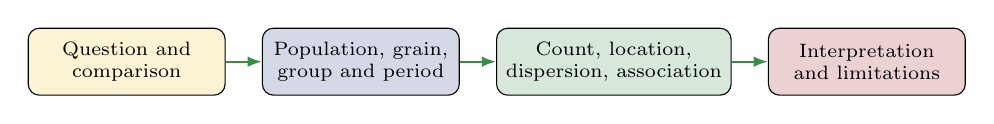
\begin{tikzpicture}[
  artifact/.style={
    draw,
    rounded corners,
    minimum width=2.50cm,
    minimum height=0.85cm,
    align=center,
    font=\scriptsize
  },
  arrow/.style={-{Latex[length=1.8mm]},thick,ukudlaGreen}
]
  \node[artifact,fill=ukudlaLightYellow] (question) {Question and\\comparison};
  \node[artifact,fill=ukudlaLightBlue,right=0.46cm of question] (scope) {Population, grain,\\group and period};
  \node[artifact,fill=ukudlaLightGreen,right=0.46cm of scope] (summary) {Count, location,\\dispersion, association};
  \node[artifact,fill=ukudlaLightRed,right=0.46cm of summary] (claim) {Interpretation\\and limitations};
  \draw[arrow] (question) -- (scope);
  \draw[arrow] (scope) -- (summary);
  \draw[arrow] (summary) -- (claim);
\end{tikzpicture}

\vspace{0.50cm}

\raggedright

\begin{itemize}
  \item The same mean can conceal different variation or skewness.
  \item A pooled summary can conceal group, batch, site or period differences.
  \item Missing values change the effective number of observations.
  \item A relationship observed in one period may not persist in another.
\end{itemize}

\vspace{0.15cm}

\begin{beamercolorbox}[rounded=true,sep=8pt]{block body}
This session moves from \textbf{motivation}, through essential \textbf{concepts}, to a reproducible \textbf{application} for analytical data.
\end{beamercolorbox}

\end{frame}
%--------------------------------------------------



\section{Concepts}


%--------------------------------------------------
% CONTENT SLIDE 3/10
\begin{frame}{Begin with the observations being described}

\small

\begin{columns}[T]

\column{0.47\textwidth}

\textbf{State the scope}

\begin{itemize}
  \item target population and observed sample;
  \item observation grain and candidate key;
  \item categorical and numerical variables;
  \item groups, periods and weighting; and
  \item missing-value rule.
\end{itemize}

\column{0.47\textwidth}

\textbf{Report the denominator}

\begin{itemize}
  \item total rows;
  \item non-missing observations;
  \item counts by relevant group and period;
  \item frequencies and proportions; and
  \item observations excluded from a statistic.
\end{itemize}

\end{columns}

\vspace{0.35cm}

\centering
\textcolor{ukudlaRed}{A statistic without its population, grouping and effective sample size is incomplete.}

\end{frame}
%--------------------------------------------------


%--------------------------------------------------
% CONTENT SLIDE 4/10
\begin{frame}{Describe location, dispersion and shape together}

\scriptsize

\begin{tabularx}{\textwidth}{lXX}
\toprule
\textbf{Feature} & \textbf{Measures} & \textbf{Interpretation and caution} \\
\midrule
Location & Mean, median, quantiles & Mean uses every value; median is less sensitive to extremes \\
Dispersion & Range, IQR, variance, standard deviation & Range depends on extremes; SD shares the variable's unit \\
Shape & Skewness, tails, modes, unusual values & Needs visual inspection; an unusual value is not automatically an error \\
Coverage & Count, missing count, proportion available & The effective sample can differ between variables and groups \\
\bottomrule
\end{tabularx}

\vspace{0.40cm}

\small

\begin{beamercolorbox}[rounded=true,sep=8pt]{block body}
Use a small set of complementary summaries. A single average cannot represent distribution, variability, coverage and shape.
\end{beamercolorbox}

\end{frame}
%--------------------------------------------------


%--------------------------------------------------
% CONTENT SLIDE 5/10
\begin{frame}{Association measures quantify co-variation}

\small

\begin{columns}[T]

\column{0.46\textwidth}

\textbf{Covariance}

\begin{itemize}
  \item sign indicates joint direction;
  \item magnitude depends on both units;
  \item sensitive to extreme observations; and
  \item difficult to compare across scales.
\end{itemize}

\column{0.49\textwidth}

\textbf{Pearson correlation}

\begin{itemize}
  \item standardizes linear co-variation;
  \item ranges from $-1$ to $1$;
  \item can hide nonlinear patterns; and
  \item changes with groups, periods and outliers.
\end{itemize}

\end{columns}

\vspace{0.35cm}

\begin{beamercolorbox}[rounded=true,sep=8pt]{block body}
Always pair association measures with a plot and the contributing observation count. Correlation is neither explanation nor causation.
\end{beamercolorbox}

\end{frame}
%--------------------------------------------------


%--------------------------------------------------
% CONTENT SLIDE 6/10
\begin{frame}{Stationarity asks whether the process remains stable}

\small

\begin{columns}[T]

\column{0.48\textwidth}

\textbf{Descriptive intuition}

Across time, ask whether:

\begin{itemize}
  \item the distribution shifts;
  \item the typical level changes;
  \item variability changes; and
  \item associations change.
\end{itemize}

\column{0.47\textwidth}

\textbf{Weak stationarity}

A time process has:

\begin{itemize}
  \item a constant mean;
  \item a constant variance; and
  \item covariance depending on lag, not calendar time.
\end{itemize}

\end{columns}

\vspace{0.30cm}

\begin{beamercolorbox}[rounded=true,sep=8pt]{block body}
Stationarity is an assumption about a data-generating process. A finite dataset can provide evidence for or against it, but cannot prove it universally.
\end{beamercolorbox}

\end{frame}
%--------------------------------------------------


%--------------------------------------------------
\section{Application}
% CONTENT SLIDE 7/10

\begin{frame}{Look for evidence of change before modeling}

\scriptsize

\begin{tabularx}{\textwidth}{lXX}
\toprule
\textbf{Pattern} & \textbf{Descriptive evidence} & \textbf{Why later models care} \\
\midrule
Trend & Period means or medians differ systematically & A constant-mean model is inappropriate \\
Changing variance & Period SDs or IQRs differ & Errors and uncertainty may not be stable \\
Structural change & An abrupt level or relationship shift & Historical parameters may not transfer \\
Seasonality/cycles & Repeated time-linked patterns & Time dependence remains in observations \\
Association drift & Correlations differ by group, site or period & One pooled slope may conceal changing relationships \\
\bottomrule
\end{tabularx}

\vspace{0.38cm}

\small

\begin{beamercolorbox}[rounded=true,sep=8pt]{block body}
Compare plots and grouped summaries across meaningful periods. Formal stationarity tests are optional extensions, not automatic verdicts.
\end{beamercolorbox}

\end{frame}
%--------------------------------------------------



%--------------------------------------------------
% CONTENT SLIDE 8/10
\begin{frame}{Describe an outcome by group and period}

\small

\begin{columns}[T]

\column{0.47\textwidth}

\textbf{For every group, report}

\begin{itemize}
  \item total and non-missing $n$;
  \item mean and median outcome;
  \item quartiles and IQR;
  \item standard deviation and range; and
  \item first and last occasion represented.
\end{itemize}

\column{0.47\textwidth}

\textbf{Compare periods}

\begin{itemize}
  \item an earlier historical period;
  \item a recent development period;
  \item a later evaluation period;
  \item levels, dispersion and coverage; and
  \item agreement with trend graphics.
\end{itemize}

\end{columns}

\vspace{0.30cm}

\centering
\textcolor{ukudlaRed}{Period summaries make potential distribution shift visible before a model is fit.}

\end{frame}
%--------------------------------------------------


%--------------------------------------------------
% CONTENT SLIDE 9/10
\begin{frame}{Describe relationships without pooling blindly}

\small
\centering

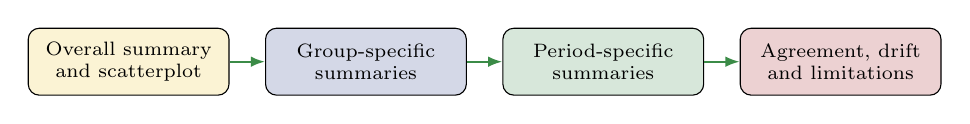
\begin{tikzpicture}[
  artifact/.style={
    draw,
    rounded corners,
    minimum width=2.55cm,
    minimum height=0.85cm,
    align=center,
    font=\scriptsize
  },
  arrow/.style={-{Latex[length=1.8mm]},thick,ukudlaGreen}
]
  \node[artifact,fill=ukudlaLightYellow] (overall) {Overall summary\\and scatterplot};
  \node[artifact,fill=ukudlaLightBlue,right=0.45cm of overall] (country) {Group-specific\\summaries};
  \node[artifact,fill=ukudlaLightGreen,right=0.45cm of country] (period) {Period-specific\\summaries};
  \node[artifact,fill=ukudlaLightRed,right=0.45cm of period] (compare) {Agreement, drift\\and limitations};
  \draw[arrow] (overall) -- (country);
  \draw[arrow] (country) -- (period);
  \draw[arrow] (period) -- (compare);
\end{tikzpicture}

\vspace{0.48cm}

\raggedright

\begin{itemize}
  \item Report each variable's location, dispersion, range and missingness.
  \item Calculate covariance and correlation with their contributing $n$.
  \item Compare pooled, group-specific and period-specific associations.
  \item Investigate whether between-group differences drive the pooled result.
  \item Retain measurement, aggregation and non-causal interpretation boundaries.
\end{itemize}

\end{frame}
%--------------------------------------------------


%--------------------------------------------------
\section{Key Message}
% CONTENT SLIDE 10/10

\begin{frame}{Key message: describe stability before modeling}

\small

\begin{columns}[T]

\column{0.47\textwidth}

\textbf{Reproducible artifacts}

\begin{itemize}
  \item descriptive-analysis script;
  \item group and period summary tables;
  \item association table with effective $n$;
  \item compact report with linked figures; and
  \item explicit grouping and missingness rules.
\end{itemize}

\column{0.47\textwidth}

\textbf{Modeling hand-off}

\begin{itemize}
  \item evidence of trends or level shifts;
  \item evidence of changing variability;
  \item stability of associations;
  \item implications for time-based splitting; and
  \item questions requiring a stated model.
\end{itemize}

\end{columns}

\vspace{0.30cm}

\begin{beamercolorbox}[rounded=true,sep=8pt]{block body}
Description does not fix non-stationarity. It reveals when later explanatory and predictive models must represent time, change or limited transferability.
\end{beamercolorbox}

\vspace{0.15cm}

\centering
\textcolor{ukudlaRed}{Summarize what was observed---and expose what may not remain stable.}

\end{frame}
%--------------------------------------------------


%--------------------------------------------------
\begin{frame}[plain,noframenumbering]{Supported by}

  South African government and the National Research Foundation

  \begin{flushleft}
    \includegraphics[trim=0cm 0cm 0cm 0cm, clip, width=0.50\textwidth]{./logos/ukudla_south_african_sponsors.pdf}
  \end{flushleft}

  German government and the German Academic Exchange Service

  \begin{flushleft}
    \includegraphics[trim=0cm 0cm 0cm 0cm, clip, width=1.00\textwidth]{./logos/ukudla_german_sponsors.pdf}
  \end{flushleft}

\end{frame}
%--------------------------------------------------

\end{document}
